\documentclass{article}
\usepackage{graphicx} % Required for inserting images
\usepackage{float} % Allows putting an [H] in \begin{figure} to specify the exact location of the figure

\title{Project 3 Writeup}
\author{Leroy S., Nikil G., Amit R,}

\begin{document}

\maketitle

\section*{The First Task}
\subsection*{Model Description}
The first task is a logistic regression problem using the binary cross entropy loss function. The model we created outputs a probability of whether the diagram is either dangerous or safe.
This probability is then compared with the threshold of 0.5 where a probability below predicts the diagram to be safe and a probability above 0.5 predicts the diagram to be dangerous. We generated an arbitrary number of diagrams and then used the Memory class which we created in order to randomly sample diagrams to process to create the training and testing datasets. 
In order to gather the input data (diagrams), for each sample in the training and testing data, we generated matrices of size 20 by 20 and randomly chose to put down a wire first as a row or col. Subsequently, we added the wires in randomly,
alternating wires being put as rows or columns. Each one of the pixels within the diagram were described in the form of a vector in the form of [A, B, C, D] where for each color, one of the variables (A, B, C, or D)
would be 1 and the others would be 0. We then flattened the diagram of 20 x 20 = 400 pixels and we got an array of length 1600 where every 4 values describes the color of each pixel. We then added the non-linear features to this feature array. \newline


\noindent The non-linear features we added to the model of the first task were constants that represented the percentage of each wire that still remained of the original color. Alternatively, it could be described as a representation
of how much each wire had been overlapped with other color wires. The idea behind these features was to create features that gave the model a more concrete idea of when each wire was placed relative to every other wire. 
These features, in turn, would theoretically allow it to predict whether certain wires were placed before others with higher accuracy. 
I calculated the percentage by finding the number of pixels of the wire’s original color that were in that row or column that the wire was placed in and dividing it by the total number of pixels in that row or column respective which in this case is always 20.
To add non-linearity, I tried functions such as the square function, tanh, and the exponential function. After comparing the increase in accuracy with respect to the model without the non-linear features, I chose the exponential function. In addition, since I didn't want the size of the features to be
too high, I chose to take the $e^{-x}$ of each non-linear feature where x is percentage of pixels of the original color for each wire This would be an array of 4 features for each wire. This would in total give a input space of 1605 including the bias term and the non-linear features. 
\newline With regards to our training model, we defined the input space to depict the features behind our wiring diagrams, each individually being represented by feature vectors composed of a constant term/bias,
a flattened representation  of the actual wiring diagram itself, and features derived from the 'findConstants' function.
We defined our output space to be a binary output (each wiring diagram assigned to either 0: safe or 1: dangerous) determined by comparing our probability output by our model to a threshold of 0.5.
To determine the architecture of our model, we utilized a logistic regression model, with our parameters given as our weights (bias and associated coefficients), learning rate $alpha$ (step size of gradient descent), epochs (num of interactions for the dataset), and our regularization parameter $lambda$ (strength of regulation to avoid overfitting).
In order to measure the loss/error of our model, we have chosen to use a binary cross-entropy function. We chose to use the binary cross-entropy loss function as we are dealing with the diagram being either dangerous or safe. Since we are dealing with two cases of which each diagram can satisfy, our problem can be categorized as a binary classification problem which makes it reasonable to use the binary cross entropy loss function. 
\[\textrm{Loss} = -\frac{1}{N} \sum_{i=1}^{N} \left[ y_i \log(p_i) + (1 - y_i) \log(1 - p_i) \right] + \frac{\lambda}{2 \times \textrm{m}} \]
The gradient is the partial derivative of the loss function. We can use this to adjust our model weights while training. We calculate this as follows:
\[
\frac{\partial J(w)}{\partial w_j} = \frac{1}{m} \sum_{i=1}^{m} (\hat{y}^{i} - y^{i}) x_j^{i}
\]
here $\hat{y}$ is calculated by: $\hat{y} = \vec{w} \cdot x^i$ \newline


\noindent We are able to use gradient descent as our training algorithm in order to train our model after calculating the gradient of the loss function. In this case, the gradient is equal to the summation of the (difference of the predicted output value (y-hat) - the actual output value symbol (y)) for each sample in the training dataset) multiplied by the j-th component (the feature that directly corresponds to j-th component of the weight array) of the input feature vector for that sample in the dataset. Y-hat is the predicted value which is the sigmoid function applied to the dot product of the weights and the input feature vector of the i-th sample. 


\[w_j = w_j - {\alpha} {\nabla} J (w_j)\]

\noindent This is the formula for which we update our weights or rather gradient descent. This formula is applied to every weight in our weight array (self.weights). This training algorithm updates the weights by taking the current weights and subtracting the value of alpha (our step size) multiplied by the gradient. The gradient symbolized by the triangle in the formula represents a vector of derivatives of the loss function with respect to each weight. 
\[\textrm{Loss} = -\frac{1}{N} \sum_{i=1}^{N} \left[ y_i \log(p_i) + (1 - y_i) \log(1 - p_i) \right] + \frac{\lambda}{2 \times \textrm{m}} \sum_{j=1}^{ \textrm{m}} w_j^2\]
L2 regularization is essentially adding the sum of the squared value of all the weights in an effort to limit the weights from becoming too large.
This, in turn, changes the gradient descent formula. When you take the gradient of the regularization term in the binary cross entropy loss formula with respect to L2 regularization, you take the derivative of the squares of each respective weight * $lambda$ /(2 * total number of weights) which gives you lambda/(total number of weights) * each weight.
\[ \frac{\partial}{\partial w_j} \left( \frac{\lambda}{2 \cdot \textrm{m}} \sum_{j=1}^{ \textrm{m}} w_j^2 \right) = \frac{\lambda}{\textrm{m}} \cdot w_j \]        
To go further in depth into this, the loss for each individual training instance is calculated utilizing logarithmic loss functions, which incorporates sigmoid. The average loss for our model is then determined by averaging each individual loss and incorporating our regularization term. In order to train our model, we implored the use of stochastic gradient descent, a training method by which in every epoch, each weight is updated after cycling through every sample in the training dataset.
Additionally, the regularization parameter $lambda$ we added to our regression model is added to this gradient to avoid overfitting. This training is repeated concurrently for the specified number of epochs given in the parameters of the model.
Within our model, we aim to avert overfitting through the implementation of L2 regularization, which penalizes our model for large weights, thus simultaneously preventing it from becoming too specialized to the given training data and improving its generalization to new data. (Implemented by adding a term proportional to the sum of the squared weights) As mentioned earlier, we controlled the regularization of our training model through the regularization parameter $lambda$ (applied to all terms except bias term). This regularization is added to the loss function throughout the duration of the model's training.

\subsubsection*{Model Analysis}
\subsubsection*{2000 data points:}
The loss graph and accuracy graph when training the model on 2000 data points is shown below:
\begin{figure}[h!]
    \centering
    \begin{minipage}{0.45\textwidth}
        \centering
        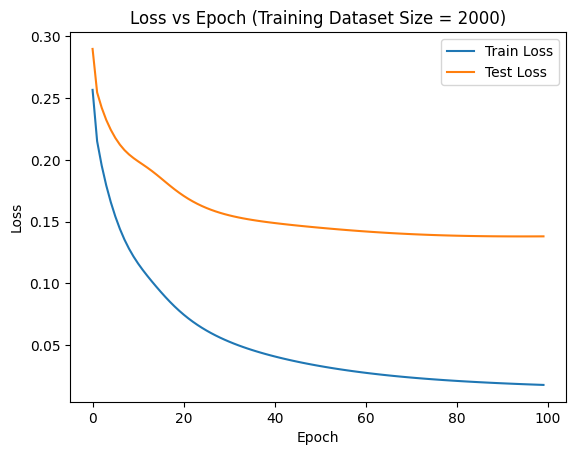
\includegraphics[width=1\textwidth]{output2000.png} % first figure itself
        \caption{Loss on 2000 data points}
    \end{minipage}\hfill
    \begin{minipage}{0.45\textwidth}
        \centering
        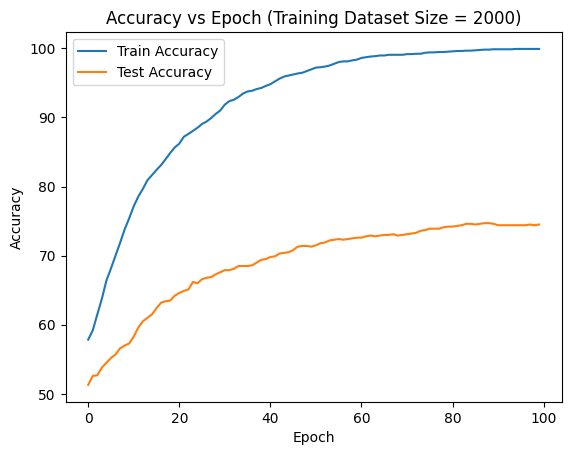
\includegraphics[width=1\textwidth]{acc2000.png} % second figure itself
        \caption{Accuracy of the model}
    \end{minipage}
\end{figure}
\newline On this model, the accuracy on the training set was 0.98 and the accuracy on the validation set was 0.74. The model was trained for 100 epochs
\subsubsection*{2500 data points:}
The loss graph and accuracy graph when training the model on 2500 data points is shown below:
\begin{figure}[h!]
    \centering
    \begin{minipage}{0.45\textwidth}
        \centering
        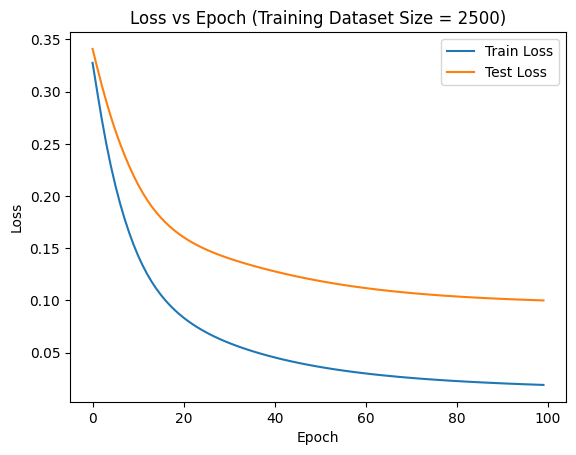
\includegraphics[width=1\textwidth]{output2500.png} % first figure itself
        \caption{Loss on 1000 data points}
    \end{minipage}\hfill
    \begin{minipage}{0.45\textwidth}
        \centering
        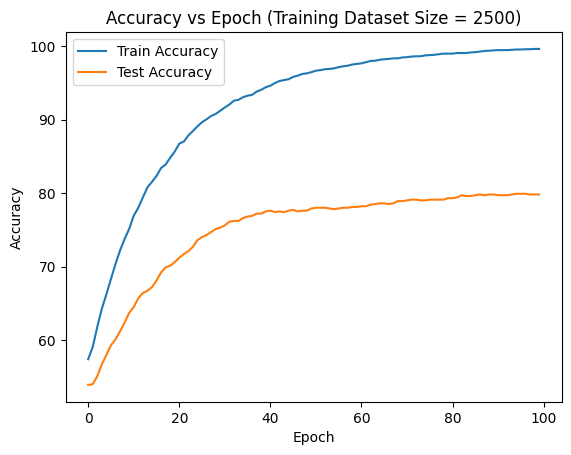
\includegraphics[width=1\textwidth]{acc2500.png} % second figure itself
        \caption{Accuracy of the model}
    \end{minipage}
\end{figure}
\newline The training accuracy is 0.98 and the validation accuracy is 0.78. The model was trained for 100 epochs
\subsubsection*{3000 data points:}
The loss graph and accuracy graph when training the model on 3000 data points is shown below:
\begin{figure}[h!]
    \centering
    \begin{minipage}{0.45\textwidth}
        \centering
        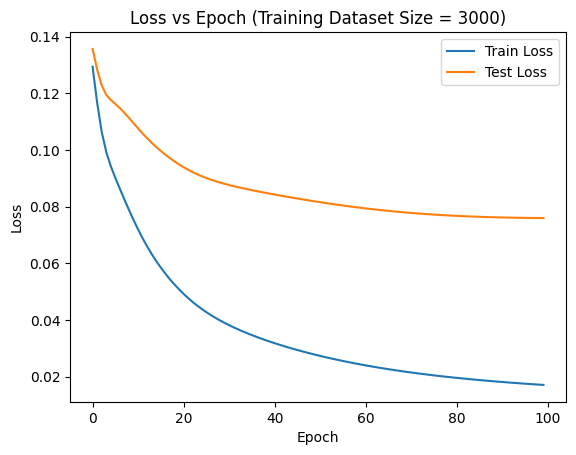
\includegraphics[width=1\textwidth]{output3000.png} % first figure itself
        \caption{Loss on 2500 data points}
    \end{minipage}\hfill
    \begin{minipage}{0.45\textwidth}
        \centering
        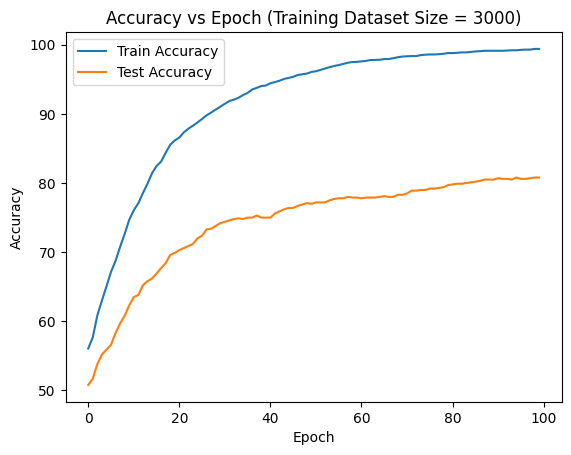
\includegraphics[width=1\textwidth]{acc3000.png} % second figure itself
        \caption{Accuracy of the model}
    \end{minipage}
\end{figure}
\newline The training accuracy is 0.96 and the validation accuracy is 0.81. The model was trained for 100 epochs
\subsubsection*{5000 data points:}
The loss graph and accuracy graph when training the model on 5000 data points is shown below:
\begin{figure}[h!]
    \centering
    \begin{minipage}{0.45\textwidth}
        \centering
        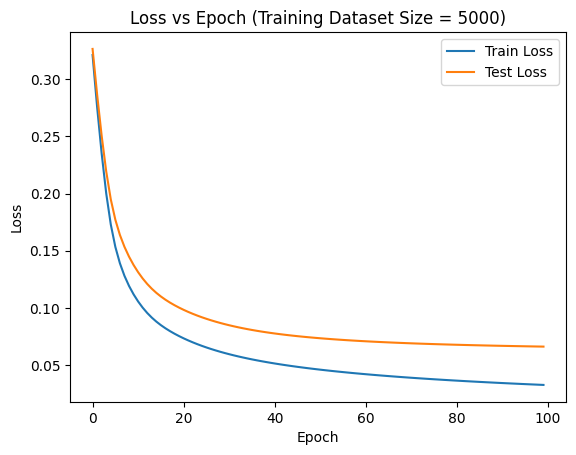
\includegraphics[width=1\textwidth]{output5000.png} % first figure itself
        \caption{Loss on 1000 data points}
    \end{minipage}\hfill
    \begin{minipage}{0.45\textwidth}
        \centering
        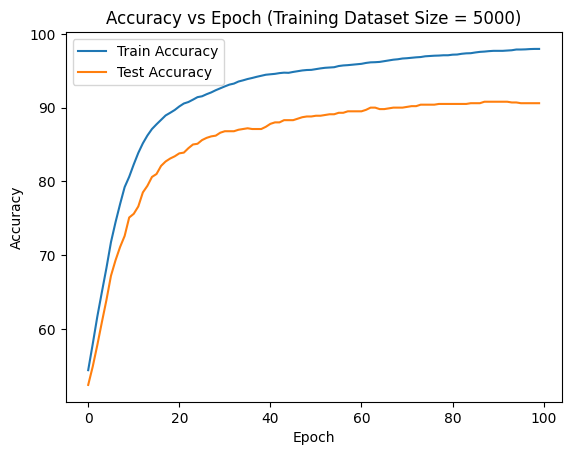
\includegraphics[width=1\textwidth]{acc5000.png} % second figure itself
        \caption{Accuracy of the model}
    \end{minipage}
\end{figure}
\newline The training accuracy is 0.96 and the validation accuracy is 0.88. The model was trained for 100 epochs\newline

\noindent As seen with the graph, there is no overfitting to be seen and the model performs well on both test and training set






\section*{The Second Task}
\subsection*{Model Description:}
The second task involved a multinomial classification problem where we had to determine, on a given dangerous wire diagram, which wire to cut.
To fulfill this purpose, we used a softmax regression model that output a number for the wire to be cut. The right wire to be cut, as stated in the project 3 writeup, would be te 3rd wire to be placed down.\newline
\newline
We numbered the wires as follows:
\begin{quote}
    \begin{enumerate}
    \item Red
    \item Blue
    \item Yellow
    \item Green
    \end{enumerate}
\end{quote}

\noindent The input space for my model is a 20x20 grid of pixels which are one hot encoded to represent the color of the wire.
This ressults into a feature vector of 1600 elements being 0 or 1. \newline

\noindent The output space for my model is a vector of 4 elements, each representing the probability of the wire being cut using the softmax function.
The wire with the highest probability is outputted as the wire to cut. Since the model is a multinomial classfication model, the softmax funtion was chosen\newline

\noindent The model space is the input space plus 4 quadratic features and 2 exponential features.
The quadratic features were obtained by first finding the total pixels each wire color occupies on the diagram. This was then passed through the function $(| x - 19 | + 2)^2$.
The exponential features were btained by considering the wires that occupied 19 pixels and then finding what wire color was present at the intersesction of these two wires. 
This was one hot encoded and then passed through the function $e^{x}$. This gave us a total of 1606 features being passed into the model\newline

\noindent The loss on my model is measured through the categorical cross entropy loss function. 
This loss function is used to measure the error between the predicted output and the actual output. The categorical cross entropy loss function is defined as follows:
\begin{equation}
    CE = -\sum_{i=1}^{N} y_{i} \log(\hat{y}_{i})
\end{equation}

\noindent Here, $y$ is the actual output and $\hat{y}$ is the predicted output. $N$ is the number of data points we have\newline

\noindent The model was trained using gradient descent. Gradient descent was fast enough by itself so it was not worth sacrificing accuracy for speed by using stochastic gradient descent.
We did gradient descent by first calculating the gradient of the loss function using partial derivatives $J(\theta)$ as follows:
\begin{equation}
    \frac{\partial J(\theta)}{\partial \theta_j} = \frac{1}{m} \sum_{i=1}^{m} (\hat{y}^i - y^i)x^i_j
\end{equation}
\noindent Here, $m$ is the number of data points and $i$ is each data point. $j$ equals to every feature. We have, $\hat{y}$ is the predicted output, $y$ is the actual output, and $x$ is the input. We then updated each weight using the formula:
\begin{equation}
    \theta_j = \theta_j - \alpha \nabla J(\theta_j)
    \end{equation}
\noindent Here, $\alpha$ is the learning rate and $\theta$ is a weight that is being changed. When calculting the giradient for bias, we just omit the multiplication of $x^i_j$
We repeat this process until the loss function is seen to converge\newline

\noindent Overfitting is often a problem when training mode
The regularization was added to the loss function using the formula:
\begin{equation}
    J(\theta) = \frac{1}{2m} \sum_{i=1}^{m} (h_\theta(x^{(i)}) - y^{(i)})^2 + \frac{\lambda}{2m} \sum_{j=1}^{n} \theta_j^2
    \end{equation}
\noindent Here, everything in the loss function remains the same. There regularization term is added at the end. In the regularization term, $\lambda$ is the regularization parameter and $n$ is the number of features.
\begin{equation}
    \frac{\partial J(\theta)}{\partial \theta_j} = \frac{1}{m} \sum_{i=1}^{m} (h_\theta(x^{(i)}) - y^{(i)})x_j^{(i)} + \frac{\lambda}{m} \theta_j
    \end{equation}
\noindent Here, everything in the gradient remains the same. The regularization term is added at the end. In the regularization term, $\lambda$ is the regularization parameter and j is the feature whose weight is being changed.
This new formula is used to update the weights in gradient descent. The regularization parameter is chosen by trying out different values and seeing which one gives the best accuracy on the validation set.\newline
\newpage
\subsection*{Model Assessment:}
\subsubsection*{500 data points:}
The loss graph and accuracy graph when training the model on 500 data points is shown below:
\begin{figure}[h!]
    \centering
    \begin{minipage}{0.45\textwidth}
        \centering
        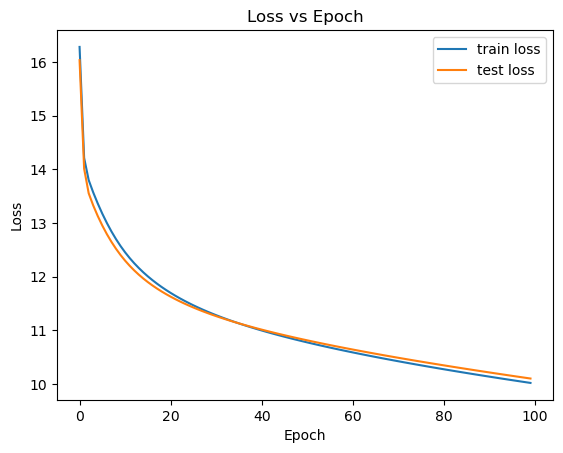
\includegraphics[width=1\textwidth]{loss_500.png} % first figure itself
        \caption{Loss on 500 data points}
    \end{minipage}\hfill
    \begin{minipage}{0.45\textwidth}
        \centering
        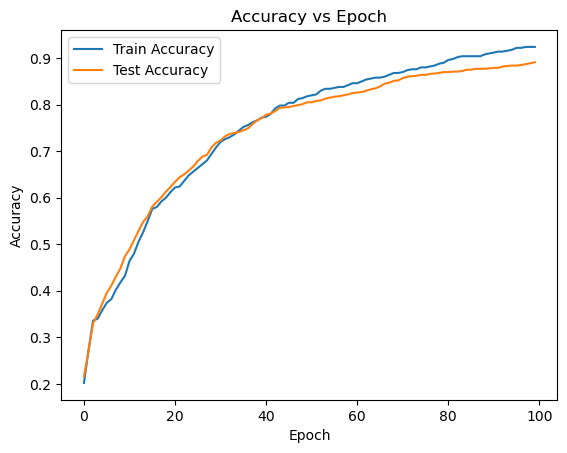
\includegraphics[width=1\textwidth]{accuracy_500.png} % second figure itself
        \caption{Accuracy of the model}
    \end{minipage}
\end{figure}
\newline On this model, the accuracy on the training set was 0.92 and the accuracy on the validation set was 0.85. The model was trained for 100 epochs
\subsubsection*{1000 data points:}
The loss graph and accuracy graph when training the model on 1000 data points is shown below:
\begin{figure}[h!]
    \centering
    \begin{minipage}{0.45\textwidth}
        \centering
        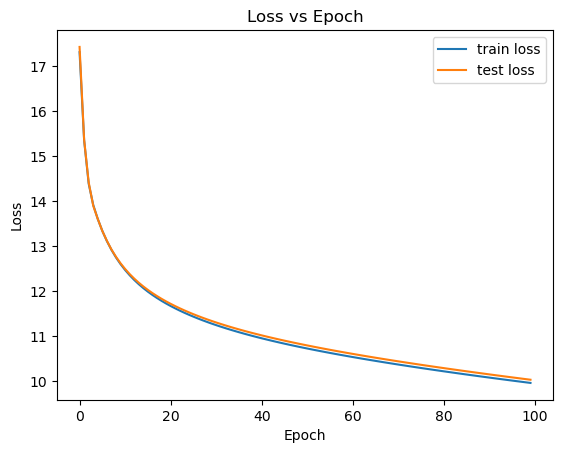
\includegraphics[width=1\textwidth]{loss_1000.png} % first figure itself
        \caption{Loss on 1000 data points}
    \end{minipage}\hfill
    \begin{minipage}{0.45\textwidth}
        \centering
        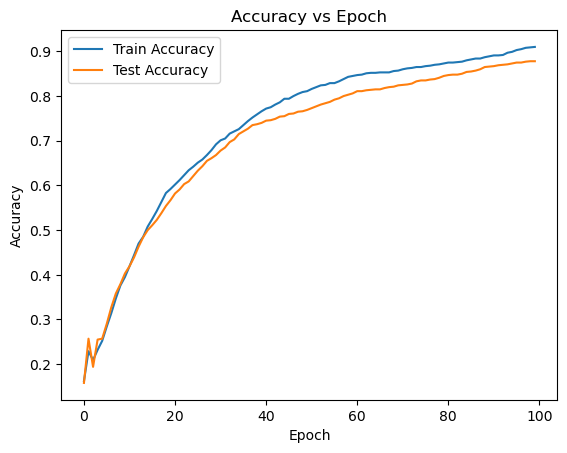
\includegraphics[width=1\textwidth]{accuracy_1000.png} % second figure itself
        \caption{Accuracy of the model}
    \end{minipage}
\end{figure}
\newline The training accuracy is 0.91 and the validation accuracy is 0.88. The model was trained for 100 epochs
\subsubsection*{2500 data points:}
The loss graph and accuracy graph when training the model on 2500 data points is shown below:
\begin{figure}[h!]
    \centering
    \begin{minipage}{0.45\textwidth}
        \centering
        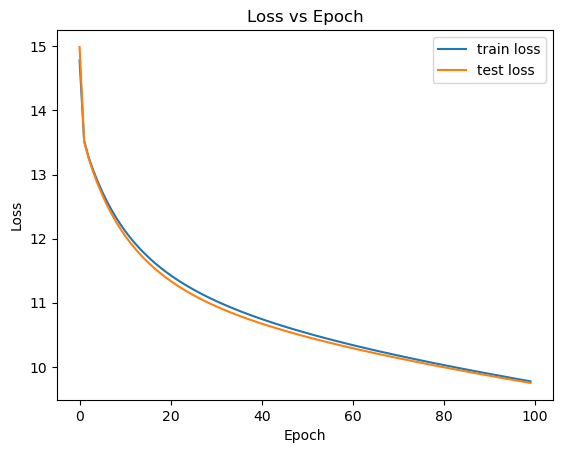
\includegraphics[width=1\textwidth]{loss_2500.png} % first figure itself
        \caption{Loss on 2500 data points}
    \end{minipage}\hfill
    \begin{minipage}{0.45\textwidth}
        \centering
        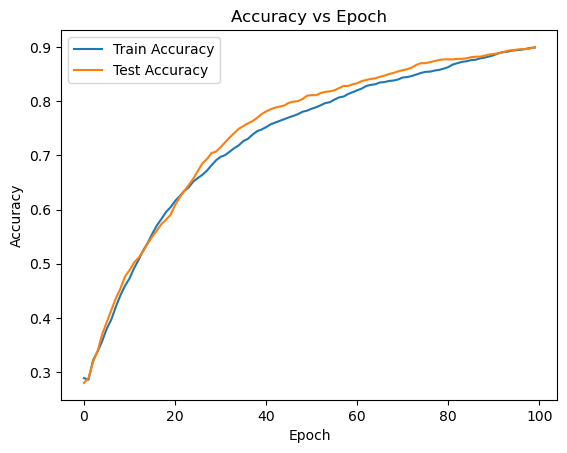
\includegraphics[width=1\textwidth]{accuracy_2500.png} % second figure itself
        \caption{Accuracy of the model}
    \end{minipage}
\end{figure}
\newline The training accuracy is 0.90 and the validation accuracy is 0.90. The model was trained for 100 epochs
\subsubsection*{5000 data points:}
The loss graph and accuracy graph when training the model on 5000 data points is shown below:
\begin{figure}[h!]
    \centering
    \begin{minipage}{0.45\textwidth}
        \centering
        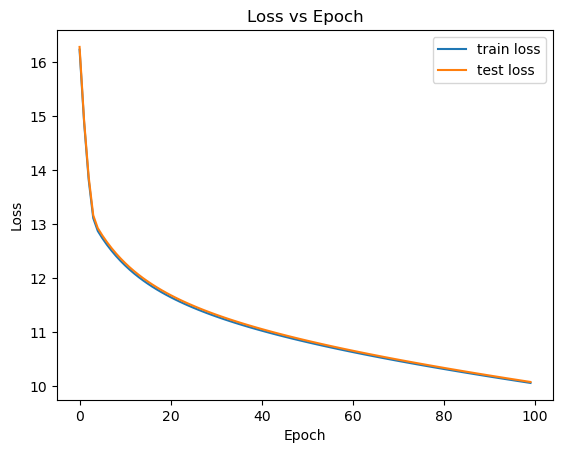
\includegraphics[width=1\textwidth]{loss_5000.png} % first figure itself
        \caption{Loss on 1000 data points}
    \end{minipage}\hfill
    \begin{minipage}{0.45\textwidth}
        \centering
        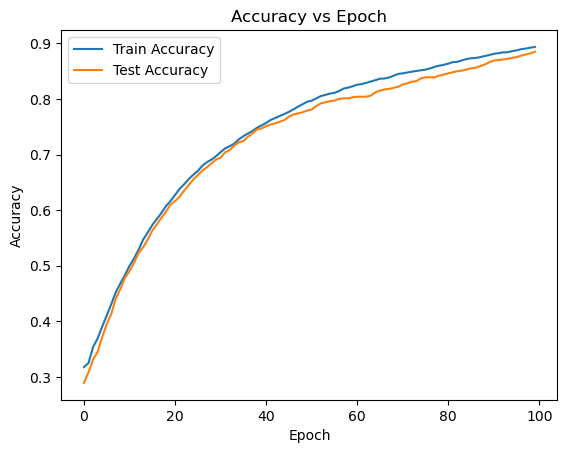
\includegraphics[width=1\textwidth]{accuracy_5000.png} % second figure itself
        \caption{Accuracy of the model}
    \end{minipage}
\end{figure}
\newline The training accuracy is 0.89 and the validation accuracy is 0.88. The model was trained for 100 epochs\newline

\noindent As seen with the graph, there is no overfitting to be seen and the model performs well on both test and training set
\subsubsection*{Getting 1.0 Accuracy on Validation Set}
It is possible to get 100\% accuracy on the validation set by training for a higher number of epochs.
Training the model on 5000 data points and for 1000 epochs, wwe get 1.0 acuuracy on both the training and testing data set. The graph for this is plotted below
\begin{figure}[H]
    \centering
    \begin{minipage}{0.45\textwidth}
        \centering
        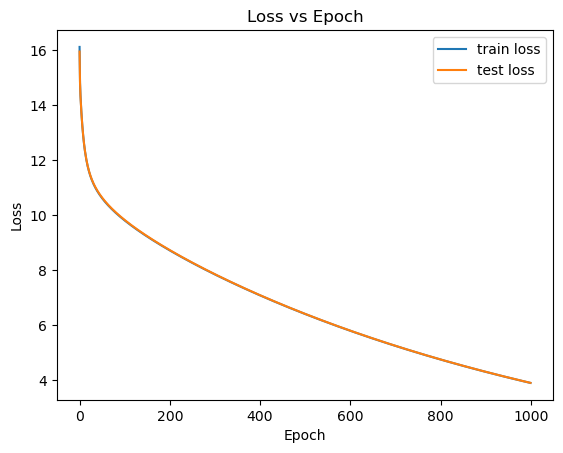
\includegraphics[width=1\textwidth]{loss_1.0.png} % first figure itself
        \caption{Loss for 5000 data points}
    \end{minipage}\hfill
    \begin{minipage}{0.45\textwidth}
        \centering
        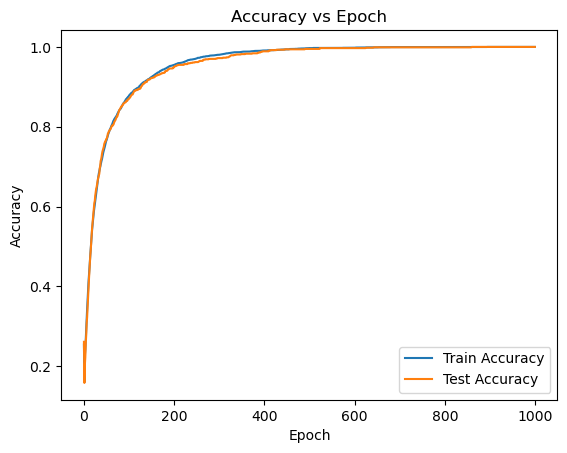
\includegraphics[width=1\textwidth]{accuracy_1.0.png} % second figure itself
        \caption{Model with 1.0 accuracy}
    \end{minipage}
\end{figure}

\noindent For datasets lower than 5000, the acuuracy is closer to 0.99 but not 1.0. We can get such high accuracy because of the features being used really help the model determine what wire is to be cut.

\newpage
\subsection*{The Bonus}
We used tensorflow to implement the model for the bonus. We created two modedls, one for part 1 and one for part 2. I combined the task of creating models uisng ML libraries and creating a minimal model in the bonus into one.

\noindent Both Models have three hidden layers. The first layer has 8 neurons, the second layer has 16 neurons and the third layer has 8 neurons. The output for model 1 is a single neuron and the output for model 2 is 4 neurons. The features being used in these models were the input diagram and the total pixels of each color present on the diagram passed through a quadratic function. After training both models the performance is listen below:
\begin{quote}
    \begin{enumerate}
    \item Training accuracy  is 0.98 and test accuracy is 0.95 for part 1
    \item Training accurcy is 0.94 and test accuracy is 0.88 for part 1
    \end{enumerate}
    \end{quote}
The loss functions for both models are shown below:
\begin{figure}[h!]
    \centering
    \begin{minipage}{0.45\textwidth}
        \centering
        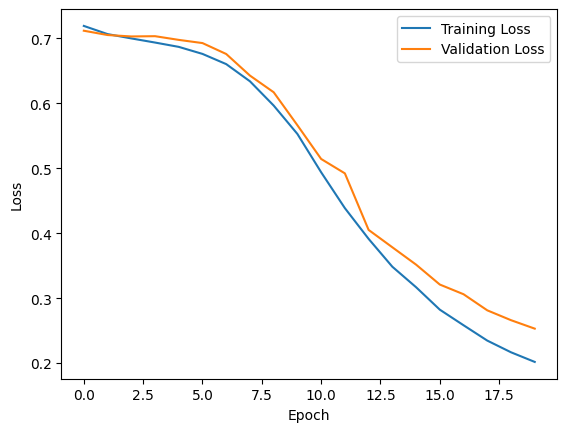
\includegraphics[width=1\textwidth]{tf_part1_loss.png} % first figure itself
        \caption{Model 1 Loss}
    \end{minipage}\hfill
    \begin{minipage}{0.45\textwidth}
        \centering
        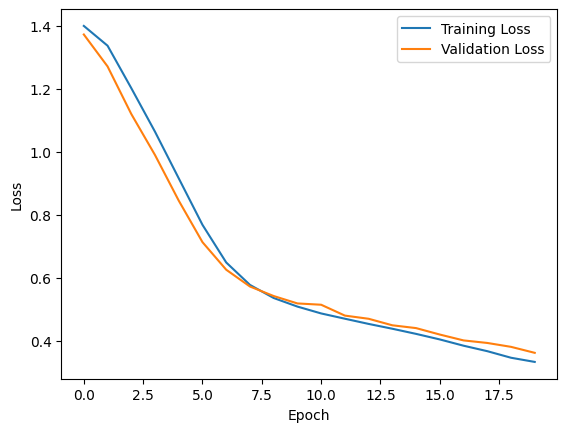
\includegraphics[width=1\textwidth]{tf_part2_loss.png} % second figure itself
        \caption{Model 2 Loss}
    \end{minipage}
\end{figure}
\end{document}